    \documentclass{article}
    
    % Use preprint option for course/project submission
    \PassOptionsToPackage{numbers,square}{natbib}
    \usepackage[preprint]{neurips_2025}

    \usepackage[utf8]{inputenc} % allow utf-8 input
    \usepackage[T1]{fontenc}    % use 8-bit T1 fonts
    \usepackage{hyperref}       % hyperlinks
    \usepackage{url}            % simple URL typesetting
    \usepackage{booktabs}       % professional-quality tables
    \usepackage{array}          % enhanced tabular features
    \usepackage{tabularx}       % expandable tables with X columns
    \usepackage{amsfonts}       % blackboard math symbols
    \usepackage{nicefrac}       % compact symbols for 1/2, etc.
    \usepackage{microtype}      % microtypography
    \usepackage{graphicx}
    \usepackage{amsmath, amssymb, amsthm}
    \usepackage{mathtools}
    \usepackage{bm}
    \usepackage{multirow}
    \usepackage{enumitem}
    \usepackage[capitalize,noabbrev]{cleveref}
    
    % Hyperref setup
    \hypersetup{
      colorlinks=true,
      linkcolor=blue,
      citecolor=blue,
      urlcolor=blue
    }
    
    % Math macros
    \newcommand{\E}{\mathbb{E}}
    \newcommand{\R}{\mathbb{R}}
    \newcommand{\norm}[1]{\left\lVert #1 \right\rVert}
    \newcommand{\inner}[2]{\left\langle #1,\,#2 \right\rangle}
    \newcommand{\KL}{\mathrm{KL}}
    \newcommand{\Var}{\mathrm{Var}}
    \newcommand{\Entropy}{\mathrm{H}}
    
    % Paper-specific macros
    \newcommand{\TAQ}{\textsc{TAQ}}
    \newcommand{\TAQO}{\textsc{TAQO}}
    \newcommand{\AWQ}{\textsc{AWQ}}
    \newcommand{\Wout}{\textsc{W\textbackslash O}}
    \newcommand\TODO[1]{\textcolor{red}{(\textbf{TODO}: #1)}}
    
    % Configure graphics search path for both local repository tree and flat Overleaf upload
    \graphicspath{{results/figures/}{figures/}{./}}
    
    \title{Computational and Memory Analysis of a Hebbian Convolutional Neural Network}
    
    \author{%
      Shay Lavi\textsuperscript{1} \quad
      Bayan Kheir\textsuperscript{1} \\
      \textsuperscript{1}Technion -- Israel Institute of Technology, Haifa, Israel \\
      \texttt{\{shay-lavi, kheir.bayan\}@campus.technion.ac.il} \quad
    }
    
    \begin{document}
    \maketitle
    \begin{abstract}

Backpropagation (BP) is the standard method for training deep neural networks, but its global backward pass requires substantial computational and memory overhead. Biologically plausible Hebbian learning offers a local alternative where synaptic updates rely only on neighboring neural activity, yet its practical resource trade-offs are rarely quantified. In this project, we develop an analytical framework to compare the hardware-independent arithmetic and memory requirements of a three-layer CIFAR-10 Hebbian convolutional network against an architecture-matched BP baseline. We evaluate multiple implementations, including direct local updates, a sparsity-aware variant, and a standard autograd substitute. Our analysis shows that a direct, sparsity-aware Hebbian implementation can reduce per-batch arithmetic operations by up to $17.7\times$ and drastically cut persistent memory compared to BP with Adam. However, these efficiency gains depend heavily on specialized sparse execution; standard automatic differentiation frameworks forfeit most of the theoretical advantage. Additionally, because the Hebbian model results in lesser accuracy, local learning demonstrates clear resource savings under constrained budgets rather than overall algorithmic superiority.
    
    % Backpropagation (BP) is the standard optimization method for deep neural networks, but its global backward pass, retained activations, gradients, and optimizer state can be computationally and memory intensive. Hebbian learning offers a biologically motivated alternative in which a synaptic update depends on local pre- and post-synaptic activity. This project asks a narrower and more testable question than whether Hebbian learning is universally ``better'': for one concrete three-layer CIFAR-10 Hebbian convolutional network, what arithmetic and memory resources are implied by the implemented learning rule, and how do they compare with an explicitly defined BP reference?
    
    % We audited the original notebooks, derived the Grossberg Instar update implemented through a PyTorch surrogate loss, and verified a direct local update against the surrogate/autograd mechanism on a deterministic three-layer batch. We then constructed three Hebbian analytical models: A1, a verified direct dense implementation; A2 conditional, a sparse-aware implementation; and B, the current dense surrogate/autograd notebook implementation. An equal-architecture BP reference was created from the limited BP facts reported by Gupta et al. and a documented set of architectural, activation, loss, and optimizer assumptions. Scalar multiplications, additions/subtractions, comparisons, divisions, square roots, and transcendental evaluations were counted separately. Persistent tensor state, analytical peak tensor payloads, one-time ZCA construction, and logical tensor movement were also modeled.
    
    % Direct electricity measurement was not used because no controlled hardware, kernel, runtime, power-sampling, or wall-clock experiment was performed. Operation counts and tensor bytes are therefore hardware-independent proxies, not joules or measured energy. At equal one-batch scope, the frozen models contain 8.667 billion operations for A1, 1.380 billion for A2 conditional, 17.268 billion for B, and 24.430 billion for BP. The one-batch BP/A2 conditional ratio is 17.699$\times$. Full method-level 20-epoch totals are 112.590 trillion for A1, 35.365 trillion for A2 conditional, 198.609 trillion for B, and 245.158 trillion for 20-epoch BP; 100-epoch BP is 1.222 quadrillion. Persistent state is estimated at 7.089~MB for A1, 0.106~MB for A2 conditional with CSR32, 10.677~MB for B, and 14.488~MB for BP with Adam.
    
    % The results show that local direct updates can remove much of the arithmetic and state associated with a global backward pass, while the current autograd implementation captures only part of that potential advantage. The largest savings belong to A2 conditional and require genuine sparse storage and kernels. Accuracy evidence also prevents a simple efficiency winner: the original paper reports 64.55\% $\pm$ 0.4 over ten runs, the saved notebook records 64.65\% for one run, and approximate comparison-paper graph reads place full-data BP above Hebbian learning at 100 epochs. Consequently, the study supports a computational-resource advantage for direct local learning under the stated models, but not a claim of lower electricity use, equal accuracy, or overall algorithmic superiority.
    \end{abstract}
    
    \vspace{1em}
    
    \section{Introduction}
    
    Modern convolutional neural networks are usually trained with backpropagation. A forward pass computes activations and a loss; a backward pass propagates derivatives through the network and accumulates parameter gradients; an optimizer then updates the parameters. This procedure is effective and general, but its learning signal is global: an early layer cannot complete its update until downstream computation and the loss derivative are available. Implementations therefore retain information from the forward pass and allocate gradient and optimizer state that do not appear in the inference-only network.
    
    Biologically inspired learning investigates alternatives to this global mechanism. Hebbian learning \cite{hebb1949organization} is organized around the principle that a connection changes according to activity at its two ends. In its simplest form, the update is proportional to the product of input and output activity:
    \begin{equation}
        \Delta w_{ij} = \eta x_j y_i
    \end{equation}

    Where $x_j$ is the pre-synaptic activation (input from neuron $j$).$y_i$ is the post-synaptic activation (output of neuron $i$).$w_{ij}$ is the synaptic weight connecting neuron $j$ to neuron $i$.$\eta > 0$ is the learning rate.
    More stable variants add competition, normalization, or a decay term. Grossberg's Instar rule \cite{grossberg1976adaptive}, used in the repository \cite{miconi2021hebbian} studied here, moves a winning neuron's weight vector toward its current input:
    \begin{equation}
    \Delta \mathbf{w}_c = \eta \sum_m y_{m,c} (\mathbf{x}_m - \mathbf{w}_c)
    \label{eq:instar_intro}
    \end{equation}
    Here $\mathbf{x}_m$ is an input patch, $y_{m,c}$ indicates whether channel $c$ wins at spatial location $m$, and $\eta$ is the learning rate. The update is local in the algorithmic sense: it uses the receptive-field input, the channel's response or winner indicator, and the channel's own weights. It does not require a label-derived error to traverse later layers.
    
    Miconi showed that convolutional Hebbian rules can be expressed as gradients of carefully chosen surrogate losses, allowing standard deep-learning frameworks to execute them efficiently \citep{miconi2021hebbian}. The associated repository contains a full CIFAR-10 implementation \citep{miconi2021repo}. Gupta et al.\ later compared BP with several biologically inspired algorithms under limited-data, limited-epoch, noise, and pruning scenarios \citep{gupta2023bio}. Their CIFAR-10 results motivate a resource comparison, particularly because Hebbian accuracy stabilizes much earlier than BP in their experiments.
    
    The practical question, however, is easy to overstate. A lower arithmetic count does not automatically indicate lower energy usage, and earlier stabilization does not imply high accuracy. Moreover, an autograd implementation of a local rule may perform work that a purpose-built local implementation would avoid. This project therefore focuses on a concrete, auditable question:
    \begin{quote}
    \itshape
    For the Hebbian CIFAR-10 CNN implementation\cite{miconi2021repo}, what compute, persistent-state, working-memory, and logical-movement costs follow from (i)~a verified direct dense Instar implementation, (ii)~a conditional sparse-aware direct implementation, and (iii)~the current surrogate/autograd implementation, compared with an explicitly documented equal-architecture BP reference?
    \end{quote}
    
    The contribution is an implementation-grounded analytical audit rather than a new training experiment. Specifically, the project:
    \begin{enumerate}[noitemsep]
    \item traces the active architecture and learning branches in existing implementations;
    \item derives the surrogate gradient and verifies a direct Instar update numerically on a deterministic three-layer batch;
    \item defines A1, A2 conditional, and B Hebbian execution models;
    \item defines a BP reference;
    \item counts scalar operation categories over matched work, configured budgets, convergence sensitivity, and fuller method-level scopes; \TODO{what the fuck is this one supposed to be}
    \item models persistent state, peak tensor payload references, ZCA construction, and logical tensor movement;
    \item places these resource results beside source-qualified accuracy evidence without constructing an artificial efficiency score.
    \end{enumerate}
    
    This scope is intentionally narrower than benchmarking runtime or power. No claim in this report converts operations into joules, bytes into electricity, or tensor payload into a measured GPU peak.
    
    \section{Background and Related Work}
    
    \subsection{Backpropagation and Global Credit Assignment}
    
    Standard BP incurs heavy computational and memory overhead. For convolutional layers, every backward pass requires two separate operations: computing gradients with respect to the weights, and propagating error gradients back to previous layers. This not only demands intensive gradient calculations, but also forces the network to cache intermediate activations until the backward pass completes, while optimizers like Adam add further memory overhead by tracking parameter moments.

    Our motivation is computational efficiency rather than biological plausibility alone. Backpropagation couples all layers through strict backward dependencies and costly global gradient updates, motivating a direct comparison with localized rules that update weights using only layer-local activity.
    
    \subsection{Hebbian Convolutional Learning Implementation}
    
    Miconi tackles the challenge of applying Hebbian learning to convolutional layers, where shared weights receive overlapping input patches \citep{miconi2021hebbian}. To avoid writing custom GPU kernels, the paper formulates surrogate loss functions whose standard PyTorch gradients mathematically reproduce classic local updates, including plain Hebbian \cite{hebb1949organization}, Grossberg Instar \cite{grossberg1976adaptive}, and Oja's rule. This trick also bypasses non-differentiable operations like Winner-Take-All (WTA): the forward pass builds a dummy computation graph, swaps in the true non-differentiable WTA outputs, and lets autograd execute the weight update.
    
    This setup is demonstrated on CIFAR-10 using a three-layer convolutional network (100, 196, and 400 filters, with a $5\times 5$ kernel in Layer 1 and $3\times 3$ kernels in Layers 2 and 3, each followed by $2\times 2$ average pooling). WTA activity governs which weights update during training, while a denser triangular-activation representation passes forward between layers for feature propagation and evaluation. Random channel pruning in the deeper layers prevents feature collapse and preserves downstream information. Once trained, the convolutional network is frozen as a fixed feature extractor, and a linear classifier trained via ridge regression on the feature representations is used to evaluate CIFAR-10 test classification accuracy \citep{miconi2021hebbian}.
    
    In summary, our goal is to determine the genuine computational and memory efficiency of Hebbian convolutional learning. The surrogate loss formulated by Miconi is fundamentally a software convenience designed to harness PyTorch's autograd engine without writing custom CUDA kernels, rather than an intrinsic requirement of the local learning rule. However, routing local updates through dense reverse-mode autograd incurs substantial algorithmic and memory overhead. Disentangling the theoretical promise of biologically inspired learning from implementation artifacts requires evaluating both the surrogate autograd pipeline and direct, purpose-built local execution.
    \subsection{Grossberg Instar} 
    
    For a filter weight vector $\mathbf{w}_c$, input patch $\mathbf{x}_m$, and learning signal $y_{m,c}$, the batched Grossberg Instar update is:

\begin{align}
\Delta \mathbf{w}_c &= \eta \sum_m y_{m,c} (\mathbf{x}_m - \mathbf{w}_c) = \eta \left[ \sum_{m \in \text{wins}(c)} \mathbf{x}_m - N_{\text{wins}}(c)\mathbf{w}_c \right]
\label{eq:instar_expanded}
\end{align}

Where $\mathbf{w}_c$ represents the current weights of filter $c$, $\Delta\mathbf{w}_c$ is the parameter update for filter $c$, $\mathbf{x}_m$ is the input patch at spatial/batch location $m$, $y_{m,c} \in \{0, 1\}$ indicates whether channel $c$ fires at patch $m$, $\eta$ is the learning rate, $\text{wins}(c)$ is the set of patch locations where channel $c$ is active, with total count $N_{\text{wins}}(c) = \vert{}\text{wins}(c)\vert{}$.

The learning signal $y_{m,c} \in \{0, 1\}$ is determined by a Winner-Take-All (WTA) competition over pre-WTA activations $a_{m,c}$:
\begin{equation}
    y_{m,c} = 
    \begin{cases} 
    1, & \text{if } a_{m,c} = \max_{k} a_{m,k} \quad \text{and} \quad a_{m,c} > 0, \\ 
    0, & \text{otherwise} 
    \end{cases}
\label{eq:wta}
\end{equation}

Under this rule, only the channel(s) achieving the maximum positive activation at patch location $m$ fire ($y_{m,c} = 1$). If the maximum activation across all channels is zero or negative, no channels fire, and non-winning channels receive no parameter update.

Writing the update in this direct form highlights why local execution is efficient: a custom implementation only needs to accumulate winning patches, apply the scaled decay term $N_{\text{wins}}(c)\mathbf{w}_c$ once per filter, and immediately free the patch memory. In contrast, the original notebook forces PyTorch autograd to compute the same result through dense forward and backward operations over the entire computation graph.

    \subsection{Gupta et al.\ Comparison Study}
    
    Gupta et al.\ compare Hebbian learning, feedback alignment, direct feedback alignment, and BP, among other algorithms \citep{gupta2023bio}. In this work, we focus on comparing Hebbian learning and BP. For their vision experiments, all methods use three convolutional layers with 100, 196, and 400 filters, followed by a linear layer for BP-like methods or a Ridge classifier for Hebbian learning. The reported BP configuration uses Adam, a batch size of 100, an initial learning rate of $10^{-5}$, a StepLR schedule (step size 1), and budgets of 20 or 100 epochs, strictly omitting regularizers such as batch normalization or dropout.

In Figure~2 of \citet{gupta2023bio}, the learning trajectories highlight differences in sample efficiency and convergence dynamics rather than ultimate accuracy parity. Particularly in restricted-data scenarios and early training phases, Hebbian learning stabilizes faster than BP; however, BP continues to improve steadily over extended training. On the full CIFAR-10 training set, Hebbian representations plateau early at roughly $66\%$ accuracy across both 20- and 100-epoch budgets, whereas BP reaches approximately $57\%$ at 20 epochs and surpasses Hebbian learning at roughly $70\%$ after 100 epochs.

    This divergence in convergence profiles motivates hybrid optimization strategies: one could leverage inexpensive Hebbian updates as an unsupervised pre-training phase until convergence, followed by BP fine-tuning for higher final accuracy.
    
    The benchmark paper does not fully specify kernels, strides, pooling, BP activations, bias choices, loss reduction, Adam beta/epsilon values, StepLR gamma, or BP preprocessing. Those omissions matter for operation counting and are handled explicitly in Section~\ref{sec:bp_reference}.
    
    \section{System and Architecture}
    
    \subsection{Active Workflow}
    
    The audited implementation is based on the reference CIFAR-10 configuration in \texttt{HebbGrad\_Github.ipynb} \cite{miconi2021repo}, which executes in four stages:
\begin{enumerate}
    \item \textbf{ZCA Whitening Preprocessing.}To prevent unsupervised Hebbian filters from collapsing onto redundant, highly correlated low-frequency patterns, ZCA whitening decorrelates input features and normalizes variance across pixels. In the notebook, this matrix is computed over a 9,000-image subset (scaled by feature dimension rather than sample count), differing from the paper's description of using the entire training set.
    \item \textbf{Unsupervised Feature Learning.} The three convolutional layers are trained with the Hebbian update rule for 20 epochs (50,000 images, batch size 100), with synaptic updates starting after an initial 201-batch burn-in phase.
\item \textbf{Representation Extraction.} A single forward pass through the frozen convolutional network extracts pooled feature representations for both the training and test sets (flattened to 1,600 dimensions per image).
\item \textbf{Linear Readout Evaluation.} An $L_2$-regularized linear model (\texttt{Ridge}) is fitted on the training representations and labels. Final CIFAR-10 test accuracy is evaluated using an $\mathrm{argmax}$ decision rule.
\end{enumerate}

Notably, the evaluation pipeline applies stochastic data augmentation (random horizontal flips) to the test set, introducing run-to-run variance even when evaluating identical frozen weights.
    
    \subsection{Architecture}
    
    Table~\ref{tab:architecture} summarizes the active CIFAR-10 network geometry and weight dimensions.
    
    \begin{table}[t]
    \centering
    \caption{Active CIFAR-10 architecture and tensor geometry for batch size 100.}
    \label{tab:architecture}
    \resizebox{\textwidth}{!}{%
    \begin{tabular}{l c l c c r l}
    \toprule
    Stage & Input tensor & Operation & \begin{tabular}[c]{@{}c@{}}Output\\(pre-pool)\end{tabular} & \begin{tabular}[c]{@{}c@{}}Output\\(post-pool)\end{tabular} & \begin{tabular}[c]{@{}r@{}}Trainable\\weights\end{tabular} & \begin{tabular}[c]{@{}l@{}}Structural\\mask\end{tabular} \\
    \midrule
    Conv 1  & $100\times 3\times 32\times 32$   & 100 filters, $5\times 5$, valid, stride 1 & $100\times 100\times 28\times 28$ & $100\times 100\times 14\times 14$ & 7,500   & Dense \\
    Conv 2  & $100\times 100\times 14\times 14$ & 196 filters, $3\times 3$, valid, stride 1 & $100\times 196\times 12\times 12$ & $100\times 196\times 6\times 6$   & 176,400 & 99\% masked \\
    Conv 3  & $100\times 196\times 6\times 6$   & 400 filters, $3\times 3$, valid, stride 1 & $100\times 400\times 4\times 4$   & $100\times 400\times 2\times 2$   & 705,600 & 99\% masked \\
    Readout & $100\times 1,600$                & Ridge to 10 one-hot targets               & $100\times 10$ scores             & ---                               & 16,010  & Dense \\
    \bottomrule
    \end{tabular}%
    }
    \end{table}
    
    The convolutional stack contains 889,500 dense weight coordinates. For the deterministic seeded masks used by the audit, 7,500 coordinates are active in layer~1, 1,771 in layer~2, and 7,142 in layer~3. Because the notebook uses dense tensors and dense \texttt{conv2d}, masked zeros do not automatically reduce its convolutional arithmetic.
    
    \subsection{Competition, Representation, and Homeostasis}
    
    A defining characteristic of Miconi's Hebbian CNN is that each convolutional layer decouples the signal driving synaptic weight updates from the signal propagated forward through the network hierarchy. In standard backpropagation architectures, the same post-activation tensor serves both downstream layer propagation and backward error gradient calculations. Here, the convolutional response bifurcates into two distinct operational pathways:
    
    \paragraph{Pre-activation and Homeostatic Balance.}
    Inputs are first standardized per sample across channels and spatial coordinates. Standard valid convolution then produces pre-activations $z_{m,c} = \mathbf{w}_c^T \mathbf{x}_m$ at patch location $m$ for channel $c$. In unsupervised competitive learning, a well-known vulnerability is the ``dead neuron'' problem, where a small subset of dominant filters with initially favorable weights win competition repeatedly while others remain dormant. To enforce competitive diversity, a learned per-channel homeostatic threshold $\theta_c$ is subtracted:
    \begin{equation}
    \tilde{z}_{m,c} = z_{m,c} - \theta_c.
    \end{equation}
    Thresholds $\theta_c$ adjust dynamically during training: channels that fire too frequently see their thresholds raised, while quiescent channels experience threshold decay. This balances filter activity around an equilibrium firing probability of approximately $1/C$ (where $C$ is the layer's channel count).
    
    \paragraph{Dual-Pathway Activation Split.}
    From this thresholded response $\tilde{z}_{m,c}$, the pipeline splits into two separate signals:
    \begin{enumerate}
        \item \textbf{Local Plasticity Signal ($y_{m,c}$):} Filter learning requires sharp, winner-take-all competition to encourage receptive field specialization. This is enforced via the hard Winner-Take-All (WTA) rule (Equation~\ref{eq:wta}), producing a sparse binary indicator $y_{m,c} \in \{0, 1\}$ where only the single channel achieving the maximum positive activation fires at location $m$. This binary signal is consumed strictly by the local Grossberg Instar rule to guide weight updates $\mathbf{w}_c$, and is immediately discarded without being passed downstream.
        \item \textbf{Forward Feature Representation ($t_{m,c}$):} Propagating an ultra-sparse binary 1-hot winner vector forward would starve deeper layers of the graded intensity and multi-feature information needed for hierarchical abstraction. Instead, forward feature propagation uses a continuous, soft-competitive ``triangle'' activation. At each spatial location $m$, each channel's thresholded response is compared against the spatial mean response across all $C$ channels, preserving only above-average activations:
        \begin{equation}
        t_{m,c} = \max\left(0, \tilde{z}_{m,c} - \frac{1}{C}\sum_{c'=1}^C \tilde{z}_{m,c'}\right).
        \label{eq:triangle}
        \end{equation}
        Unlike the winner-take-all signal, multiple channels can be active simultaneously under this rectified triangular activation, retaining graded feature intensities for downstream layers.
    \end{enumerate}
    
    Finally, the continuous activation tensor $t$ undergoes $2\times 2$ average pooling to downsample spatial dimensions before entering the next convolutional layer. In Layer~3, the pooled representation ($100 \times 400 \times 2 \times 2 = 1,600$ features per sample) forms the final feature vector evaluated by the linear Ridge readout.

    \section{Hebbian Implementation Analysis}
    
    \subsection{Surrogate Autograd Mechanism}
    
    For a filter $\mathbf{w}_c$ and patch $\mathbf{x}_m$, let the linear convolution output be $z_{m,c} = \mathbf{w}_c^T \mathbf{x}_m$. The notebook constructs
    \begin{align}
    y^{\text{grad}}_{m,c} &= z_{m,c} - \frac{1}{2} \|\mathbf{w}_c\|_2^2, \\
    L &= -\frac{1}{2} \sum_{m,c} (y^{\text{grad}}_{m,c})^2.
    \end{align}
    Its analytical derivative is
    \begin{align}
    \frac{\partial y^{\text{grad}}_{m,c}}{\partial \mathbf{w}_c} &= \mathbf{x}_m - \mathbf{w}_c, \\
    \frac{\partial L}{\partial \mathbf{w}_c} &= -\sum_m y^{\text{grad}}_{m,c} (\mathbf{x}_m - \mathbf{w}_c).
    \end{align}
    Before \texttt{backward()}, the notebook replaces the forward value of $y^{\text{grad}}$ with the binary WTA tensor while retaining the original graph. Standard SGD therefore applies
    \begin{equation}
    \Delta \mathbf{w}_c = -\eta \frac{\partial L}{\partial \mathbf{w}_c} = \eta \sum_m y^{\text{WTA}}_{m,c} (\mathbf{x}_m - \mathbf{w}_c),
    \end{equation}
    which is Grossberg Instar. The global-looking \texttt{loss.backward()} is thus a convenient way to ask PyTorch for a local update; it does not make the mathematical learning signal equivalent to supervised BP.
    
    \subsection{Deterministic Equivalence Test}
    
    \texttt{direct\_hebb\_equivalence\_test.py} compares two implementations on the same deterministic float32 batch:
    \begin{itemize}[noitemsep]
    \item the notebook-style surrogate expression, value replacement, autograd, and SGD step;
    \item a direct Instar accumulation without autograd.
    \end{itemize}
    The test includes all learning-relevant active branches: per-sample normalization, the three convolutional shapes, top-1 binary WTA, triangle activations, average pooling, layer learning rates, seeded structural masks, filter normalization, and adaptive-threshold updates. It uses a post-burn-in batch because an initial burn-in batch would perform no optimizer step and would not test update equivalence.
    
    For all three layers, the test reports zero maximum and mean absolute differences for both updated weights and thresholds within $\text{atol} = 10^{-6}$ and $\text{rtol} = 10^{-5}$. It also verifies the expected shapes. This particular deterministic batch happened to produce exactly one positive WTA entry per spatial column; that observation is not a generic property of the active cutoff-and-binarization implementation. This establishes numerical equivalence for the tested batch and branches. Together with the algebra above, it supports the direct-update model. It does \textbf{not} demonstrate a complete A1 or A2 conditional training run, reproduce end-to-end accuracy, validate sparse kernels, or prove that every stochastic trajectory is bitwise identical.
    
    \subsection{Three Hebbian Execution Models}
    
    \paragraph{A1 --- Verified Direct/Local Dense Model.} A1 uses dense weights and dense forward convolutions but computes Instar directly. It therefore removes the surrogate graph, dense convolution weight-gradient, and parameter-gradient buffers. The active structural mask is still applied densely in layers~2 and~3. A1 is the strongest model directly supported by the update equivalence test while retaining conventional dense convolution.
    
    \paragraph{A2 Conditional --- Sparse-Aware Direct/Local Model.} A2 conditional applies the same Instar mathematics but assumes sparse storage for the masked higher-layer filters and specialized kernels that skip every masked coordinate during convolution, accumulation, masking, and normalization. Layer~1 remains dense. The model remains conditional: neither the notebook nor standard dense \texttt{conv2d} realizes these savings automatically, and the project did not implement or benchmark such kernels.
    
    \paragraph{B --- Current Surrogate/Autograd Model.} B represents the active notebook mechanism: dense forward convolution, surrogate expression and loss, dense autograd weight-gradient computation, SGD update, dense masks, filter normalization, and threshold adaptation. It remains Hebbian in its mathematical update, but its execution includes reverse-mode machinery introduced for implementation convenience.
    
    Keeping these models separate prevents two common errors: calling the current notebook a hand-optimized local implementation, and attributing hypothetical sparse savings to dense PyTorch execution.
    
    \section{Backpropagation Reference}
    \label{sec:bp_reference}
    
    To evaluate backpropagation under an identical architectural budget, we establish a deterministic reference implementation and an exact analytical cost model. The baseline comprises 905,510 trainable parameters across three convolutional stages and a linear head, projecting the final $400 \times 2 \times 2$ representation into a 10-class output.
    
    Table~\ref{tab:bp_assumptions} outlines the baseline specification, distinguishing parameters explicitly stated by \citet{gupta2023bio} from the architectural choices required for analytical evaluation.

\begin{table*}[t]
\centering
\small
\renewcommand{\arraystretch}{1.15}
\caption{Backpropagation baseline specification: reported parameters versus benchmark assumptions.}
\label{tab:bp_assumptions}
\begin{tabularx}{\textwidth}{l l >{\raggedright\arraybackslash}X}
\toprule
Specification Item & Source & Baseline Implementation \\
\midrule
Dataset \& channel counts & Reported & CIFAR-10; 100, 196, and 400 convolutional channels \\
Classifier head & Reported & Trainable linear layer ($1{,}600 \to 10$) \\
Optimizer & Reported & Adam \\
Batch size \& initial learning rate & Reported & 100 and $1\times 10^{-5}$ \\
Training budget & Reported & 20 or 100 epochs \\
Learning rate schedule & Inferred & StepLR ($\text{step size}=1$, assumed decay factor $\gamma = 0.95$) \\
Regularization & Reported & No batch normalization, dropout, or auxiliary regularizers \\
Kernels, strides, pooling & Matched & Matched to Hebbian pipeline: $5\times 5$, $3\times 3$, $3\times 3$ valid convolutions; $2\times 2$ average pooling \\
Activation functions & Assumed & Standard ReLU after each convolution \\
Convolutional biases & Matched & Disabled to match Hebbian layer formulation \\
Classifier bias & Assumed & Enabled \\
Loss function & Standard & Mean cross-entropy \\
Adam hyperparameters & Standard & PyTorch defaults: $\beta_1=0.9$, $\beta_2=0.999$, $\epsilon=10^{-8}$, no weight decay \\
Input preprocessing & Standard & Standardized per-sample normalization (matching Hebbian input dimensions) \\
\bottomrule
\end{tabularx}
\end{table*}

The baseline was validated using deterministic inputs: intermediate tensor geometries strictly matched the layer specifications in Table~\ref{tab:architecture}, loss evaluation remained stable, and full forward-backward update steps executed without gradient anomalies. This verification confirms the structural and numerical consistency of our analytical model. Finally, we note that the post-training pruning evaluated by \citet{gupta2023bio} does not reduce training operation counts, as pruning is applied strictly after training completes.

    \section{Computational-Cost Methodology}
    
    \subsection{Why Operation Counts Rather than Electricity}
    
    Electricity depends on hardware, precision, clocking, kernel selection, memory hierarchy, parallel utilization, compiler and library versions, cooling and power-delivery overhead, and measurement protocol. None of these variables was experimentally controlled in this project. Converting a scalar operation into a fixed energy constant would create false precision.
    
    Instead, the analysis counts scalar work implied by explicit reference formulas. This is hardware-independent and reproducible, but it is not a timing or energy model. A fused GPU kernel may issue fewer instructions than the scalar expansion; another implementation may move more data or launch more kernels. The correct interpretation is comparative algorithmic workload under shared counting conventions.
    
    \subsection{Counted Categories}
    
    The models track:
    \begin{itemize}[noitemsep]
    \item multiplications;
    \item additions and subtractions;
    \item comparisons;
    \item divisions;
    \item square roots; and
    \item for BP cross-entropy, exponential and logarithmic evaluations as transcendental operations.
    \end{itemize}
    
    ``Basic FLOPs'' means multiplications plus additions/subtractions. ``Total scalar operations'' adds all listed categories with unit weight. That aggregation is convenient for tables, but it does not imply that a square root, comparison, division, and multiplication have equal latency or energy on real hardware.
    
    Dense convolution is expanded as one dot product per output activation. With $A$ output activations and input dimension $D$, it uses $A\cdot D$ multiplications and $A\cdot (D-1)$ additions. Top-1 competition uses $C-1$ comparisons per spatial column. A $2\times 2$ average-pooling output uses three additions and one division. Normalization is modeled with a centered two-pass scalar convention rather than a library-specific fused kernel.
    
    For BP, the model includes forward convolution, ReLU, pooling, pooling backward, ReLU backward, convolutional weight gradients, convolutional input gradients where required, the linear classifier, stable mean cross-entropy, and Adam. The Adam reference counts six multiplications, four additions/subtractions, three divisions, and one square root per parameter.
    
    \subsection{Burn-in and Representative-Batch Assumptions}
    
    The notebook initializes \texttt{nbbatches} at $-1$ and updates weights only when $\texttt{nbbatches} > 200$. Therefore the 20-epoch schedule contains 10,000 batches but 9,799 optimizer-update batches. Forward, normalization, competition, triangle, pooling, and threshold work still occur during burn-in; weight-update, mask, and normalization work follow the source branch schedule.
    
    Winner-dependent direct Instar counts use the deterministic reference batch, which happened to contain exactly one positive WTA winner at every spatial column. The generic implementation can instead produce zero winners for a non-positive maximum or multiple winners for a positive tie at the cutoff. Epoch totals retain the frozen assumption that the deterministic batch's winner count is representative, and A2 conditional also assumes that the reference pairing between winners and nonzero mask coordinates is representative. These are analytical estimates, not measurements of every training batch.
    
    \subsection{Comparison Scopes}
    
    The project reports several scopes because no single total answers every question:
    \begin{enumerate}[noitemsep]
    \item \textbf{Representative one batch.} A post-burn-in training batch, with matched network geometry and preprocessing excluded from all methods in the direct BP comparison.
    \item \textbf{Equal 20 epochs.} Each method processes 10,000 training batches. This is the cleanest equal-work training-core comparison.
    \item \textbf{Configured budgets.} Hebbian learning uses its active 20 epochs while BP uses the comparison paper's 100-epoch budget. This is a protocol comparison, not equal accuracy.
    \item \textbf{Convergence sensitivity.} Hebbian totals are scaled to approximately five epochs and compared with 100-epoch BP because Gupta et al.\ describe this stabilization pattern. This is explicitly \textbf{not} an equal-accuracy comparison.
    \item \textbf{Full method-level subtotal.} Hebbian totals include known ZCA construction arithmetic, Hebbian training, 50,000-example training-feature collection, 10,000-example test-feature collection, Ridge fitting, and Ridge evaluation. BP totals include supervised training and a 10,000-example test pass.
    \end{enumerate}
    
    \subsection{ZCA and Ridge}
    
    The active notebook builds ZCA from 9,000 images with 3,072 features. After per-image centering and standardization, its code forms $\mathbf{T}^T \mathbf{T}$ and divides by $\texttt{t.shape[1]} = 3072$, not by the 9,000 samples. The matrix entering regularization and eigendecomposition is therefore a scaled scatter matrix rather than a conventional sample covariance. The known arithmetic around normalization, this scaled scatter-matrix construction, diagonal regularization, inverse-square-root eigenvalue transformation, matrix reconstruction, and auxiliary projections is counted. The dense symmetric eigensolver is not assigned an exact count because \texttt{torch.symeig} does not fix the driver, reduction strategy, convergence behavior, or backend. Instead, a broad $(4/3)F^3$ to $10F^3$ sensitivity range is reported: $\approx 3.87\times 10^{10}$ to $\approx 2.90\times 10^{11}$ basic operations for $F = 3072$. Adding this range changes the Hebbian method totals by only 0.019\% to 0.820\%, depending on the model, and does not change their ordering.
    
    The notebook calls default \texttt{Ridge()} without pinning a scikit-learn version. The main analytical reference assumes a dense primal Cholesky path. The fitting phase contributes $\approx 2.59\times 10^{11}$ modeled operations, while test prediction and evaluation contribute $\approx 3.20\times 10^{8}$ operations.
    
    \section{Memory and Resource Methodology}
    
    \subsection{Persistent Learning State}
    
    Persistent state is the payload that must remain across training steps. Depending on the method, it includes dense or sparse parameters, masks or sparse indices, parameter gradients, optimizer state, and Hebbian thresholds. Values are decimal MB and assume FP32 tensor values. A2 conditional uses FP32 values plus int32 CSR column indices and row pointers for higher-layer sparse filters.
    
    A1 needs dense weights, higher-layer masks, and thresholds but no gradient or optimizer tensors. B retains dense weights, dense masks, parameter gradients, and thresholds. BP retains parameters, gradients, and two Adam moment tensors. These differences expose an advantage of local direct updates that is separate from operation count.
    
    \subsection{Working-Memory References}
    
    Peak-memory figures are analytical liveness inventories, not allocator measurements. A1 and A2 conditional can update one layer and discard local learning intermediates before proceeding. B must support the surrogate graph and autograd payloads. BP must retain forward information until a global backward pass and requires transient activation-gradient storage.
    
    The BP values are alternative references rather than additive terms:
    \begin{itemize}[noitemsep]
    \item retained-forward baseline;
    \item an optimized reference with one recycled largest activation-gradient buffer; and
    \item a conservative two-gradient-buffer envelope with no assumed early release of forward saves.
    \end{itemize}
    
    \subsection{ZCA Construction and Logical Movement}
    
    ZCA construction is a one-time preprocessing phase and is kept separate from ordinary per-batch training. In the active code, the $9000\times 3072$ normalized data matrix produces a $3072\times 3072$ scaled scatter matrix through $\mathbf{T}^T \mathbf{T} / 3072$. The source-visible peak includes the sample tensors and multiple $3072\times 3072$ matrices. After construction, ordinary Hebbian processing retains the 37.749~MB ZCA matrix rather than the full construction peak.
    
    Logical tensor movement counts idealized whole-tensor reads and writes under the model's reuse assumptions. It is neither physical DRAM traffic nor a hardware bandwidth measurement. Cache behavior, tiling, fusion, sparse format conversion, transfers, and allocator behavior can substantially change actual traffic.
    
    \section{Results}
    
    \subsection{Matched-Work Training-Core Compute}
    
    \begin{figure}[htbp]
    \centering
    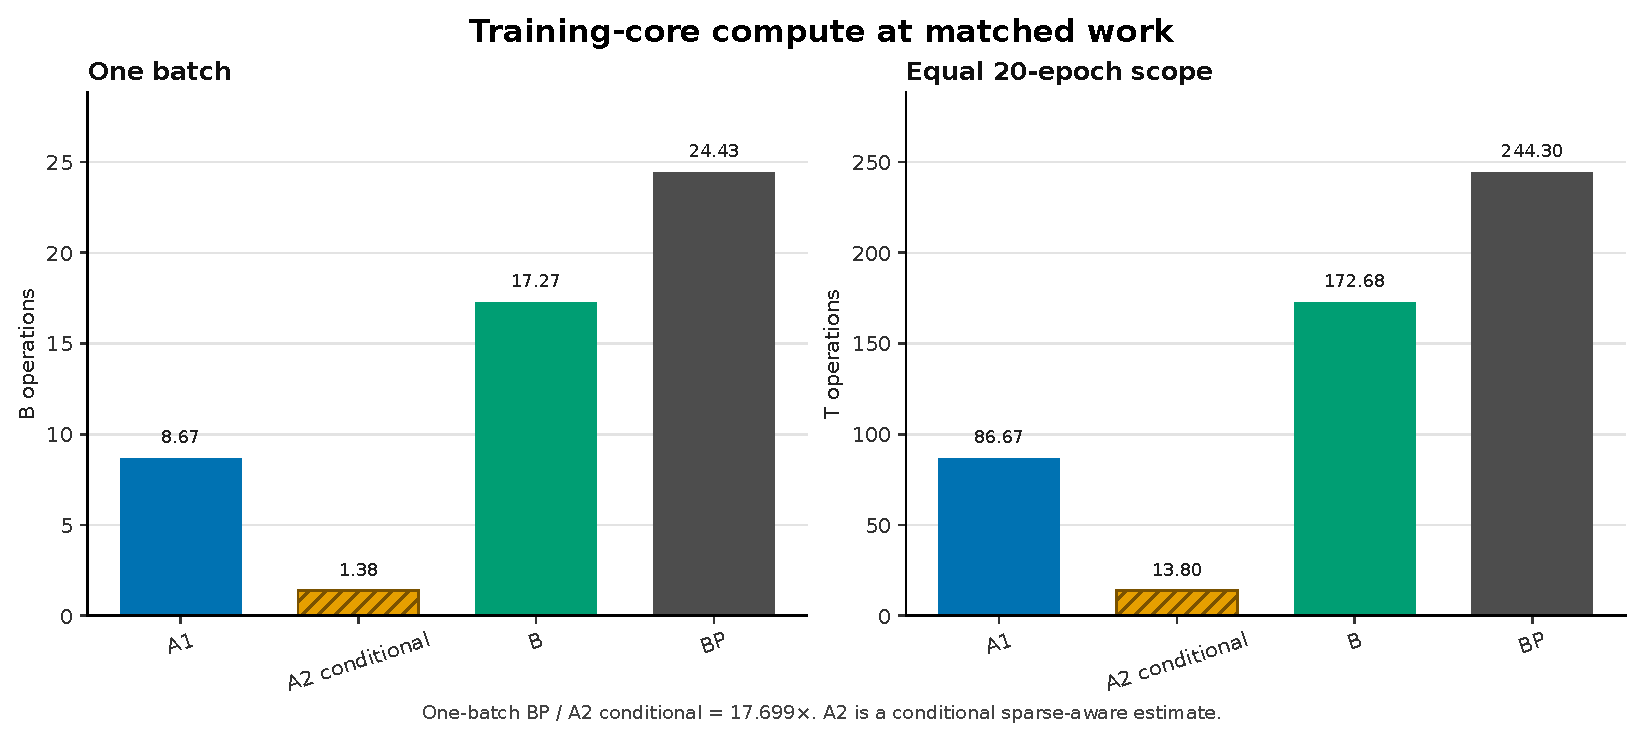
\includegraphics[width=0.88\linewidth]{fig01_compute_same_work}
    \caption{Analytical training-core operations for one representative post-burn-in batch and for equal 20-epoch scope. A2 conditional is a sparse-aware model. Preprocessing is excluded consistently from the direct BP comparison.}
    \label{fig:compute_same_work}
    \end{figure}
    
    Figure~\ref{fig:compute_same_work} isolates the learning core under matched work. For one batch, A1 requires $\approx 8.67 \times 10^9$ scalar operations, A2 conditional requires $\approx 1.38 \times 10^9$, B requires $\approx 17.27 \times 10^9$, and BP requires $\approx 24.43 \times 10^9$. The corresponding equal-20-epoch totals are $\approx 86.67 \times 10^{12}$ for A1, $\approx 13.80 \times 10^{12}$ for A2 conditional, $\approx 172.68 \times 10^{12}$ for B, and $\approx 244.30 \times 10^{12}$ for BP.
    
    \begin{table}[t]
    \centering
    \small
    \renewcommand{\arraystretch}{1.15}
    \caption{Headline matched-work training-core totals.}
    \label{tab:headline_compute}
    \begin{tabularx}{\textwidth}{l c c >{\raggedright\arraybackslash}X}
    \toprule
    Method & One batch & Equal 20 epochs & Interpretation \\
    \midrule
    A1 direct dense              & $\approx 8.67 \times 10^9$  & $\approx 86.67 \times 10^{12}$  & Verified direct update, dense convolution \\
    A2 conditional sparse-aware  & $\approx 1.38 \times 10^9$  & $\approx 13.80 \times 10^{12}$  & Requires genuine sparse storage and kernels \\
    B surrogate/autograd         & $\approx 17.27 \times 10^9$ & $\approx 172.68 \times 10^{12}$ & Current dense notebook execution model \\
    BP                           & $\approx 24.43 \times 10^9$ & $\approx 244.30 \times 10^{12}$ & Equal-architecture analytical reference \\
    \bottomrule
    \end{tabularx}
    \end{table}
    
    The one-batch BP/A1 ratio is about 2.819, BP/A2 conditional is 17.699, and BP/B is about 1.415. The result explains two different effects. First, direct Instar avoids much of BP's backward and Adam work. Second, the current surrogate/autograd implementation B spends substantially more than A1 because it expresses the local rule through dense reverse-mode machinery. A2 conditional gains a further large reduction only by treating structural zeros as absent work.
    
    \subsection{Training Budgets and Convergence Sensitivity}
    
    \begin{figure}[htbp]
    \centering
    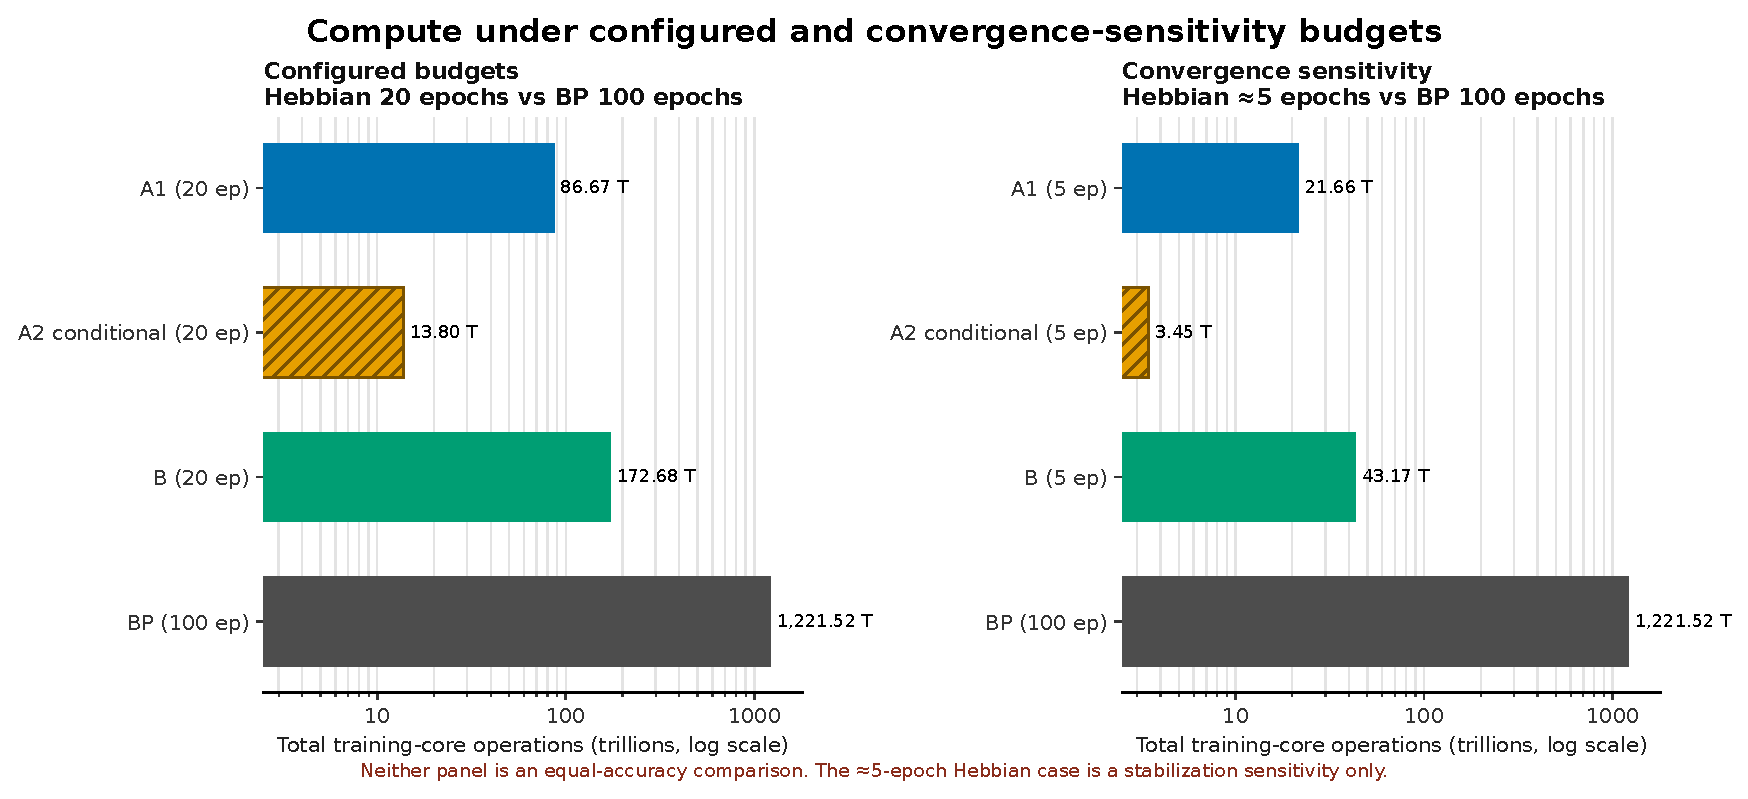
\includegraphics[width=0.92\linewidth]{fig02_compute_training_budgets}
    \caption{Training-core totals under configured Hebbian-20/BP-100 budgets and under the Hebbian-approximately-5/BP-100 convergence sensitivity. The logarithmic axis supports scale comparison. Neither panel is accuracy matched.}
    \label{fig:compute_training_budgets}
    \end{figure}
    
    At configured budgets, 100-epoch BP requires $\approx 1.22 \times 10^{15}$ modeled operations, compared with $\approx 86.67 \times 10^{12}$ for A1, $\approx 13.80 \times 10^{12}$ for A2 conditional, and $\approx 172.68 \times 10^{12}$ for B at 20 epochs. The BP totals are therefore about 14.095 times A1, 88.517 times A2 conditional, and 7.074 times B.
    
    If the comparison paper's qualitative stabilization statement is applied as a sensitivity budget, five-epoch Hebbian totals are $\approx 21.66 \times 10^{12}$ for A1, $\approx 3.45 \times 10^{12}$ for A2 conditional, and $\approx 43.17 \times 10^{12}$ for B. The 100-epoch BP total is then 56.393, 354.339, and 28.296 times larger, respectively. These ratios show how strongly training budget can dominate cumulative arithmetic. They must not be read as ``Hebbian reaches BP's 100-epoch accuracy in five epochs'': the source accuracy plot does not support that claim.
    
    \subsection{Full Method-Level Compute}
    
    \begin{figure}[htbp]
    \centering
    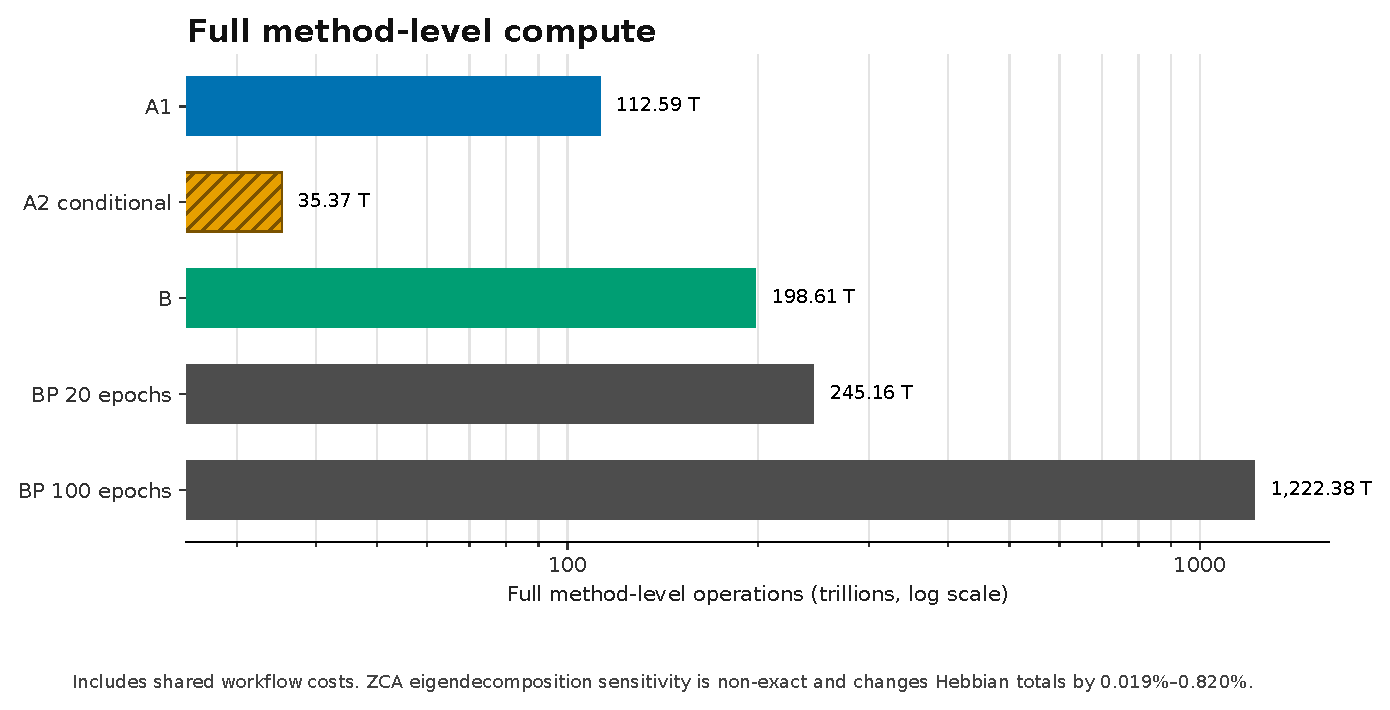
\includegraphics[width=0.88\linewidth]{fig03_compute_method_level}
    \caption{Full method-level analytical subtotals. Hebbian rows include known ZCA arithmetic, 20 training epochs, post-training train/test feature extraction with convolutional weights frozen while adaptive thresholds continue to update, Ridge fitting, and evaluation. The ZCA eigensolver is treated separately as a sensitivity range.}
    \label{fig:compute_method_level}
    \end{figure}
    
    The fuller method-level scope produces $\approx 112.59 \times 10^{12}$ operations for A1, $\approx 35.37 \times 10^{12}$ for A2 conditional, and $\approx 198.61 \times 10^{12}$ for B. BP totals are $\approx 245.16 \times 10^{12}$ at 20 epochs and $\approx 1.22 \times 10^{15}$ at 100 epochs.
    
    Adding feature extraction and Ridge narrows the gap between the direct Hebbian training core and the overall method because those downstream stages are shared by all three Hebbian execution models. Even so, the ordering is unchanged. The B subtotal remains below 20-epoch BP, but much closer than A1 and especially A2 conditional.
    
    \subsection{Persistent State}
    
    \begin{figure}[htbp]
    \centering
    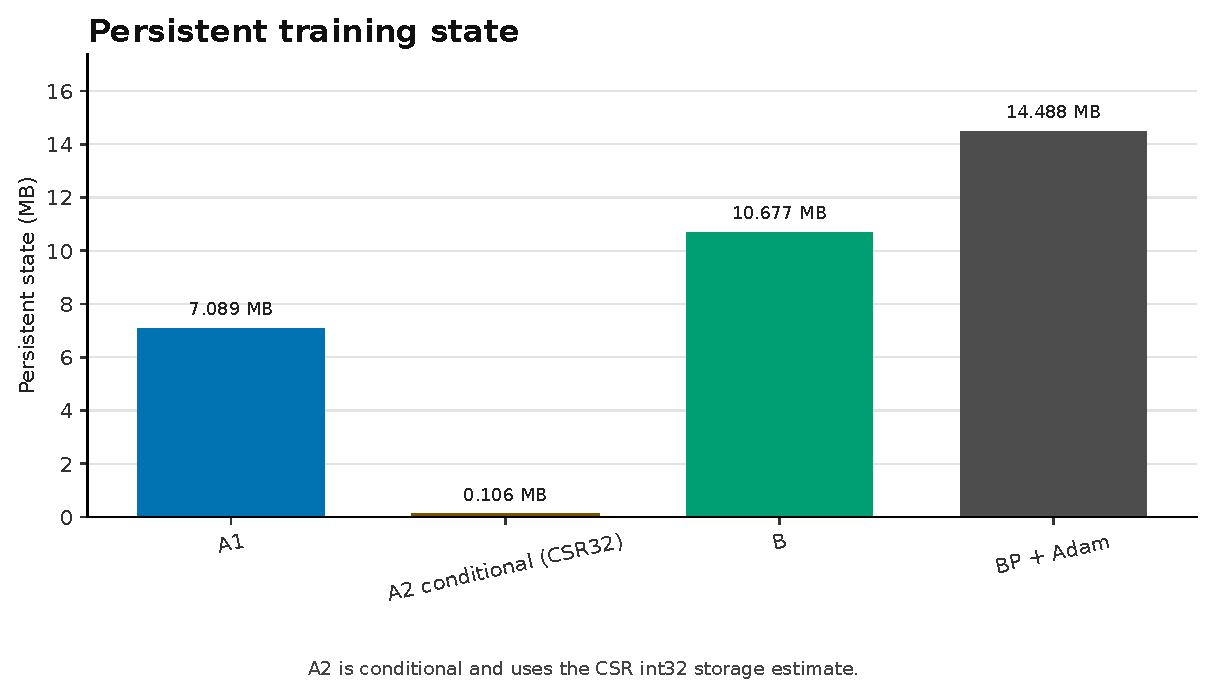
\includegraphics[width=0.85\linewidth]{fig04_memory_persistent_state}
    \caption{Persistent tensor payloads in decimal MB. A2 conditional uses a CSR32 sparse representation; BP includes parameter gradients and two Adam moment tensors.}
    \label{fig:memory_persistent_state}
    \end{figure}
    
    Persistent state is estimated at 7.089~MB for A1, 0.106~MB for A2 conditional, 10.677~MB for B, and 14.488~MB for BP. The A2 conditional figure is a total persistent-state value: it includes sparse parameter-representation storage, CSR metadata, and Hebbian thresholds. The BP total is driven by 3.622~MB of parameters, 3.622~MB of gradients, and 7.244~MB of Adam moments. B needs dense parameter gradients because autograd is used, even though the mathematical rule is local. A1 removes those gradients but still stores dense weights and higher-layer masks. A2 conditional is small because it stores only active higher-layer values and CSR metadata in addition to its thresholds.
    
    \subsection{Peak-Memory References and ZCA Construction}
    
    \begin{figure}[htbp]
    \centering
    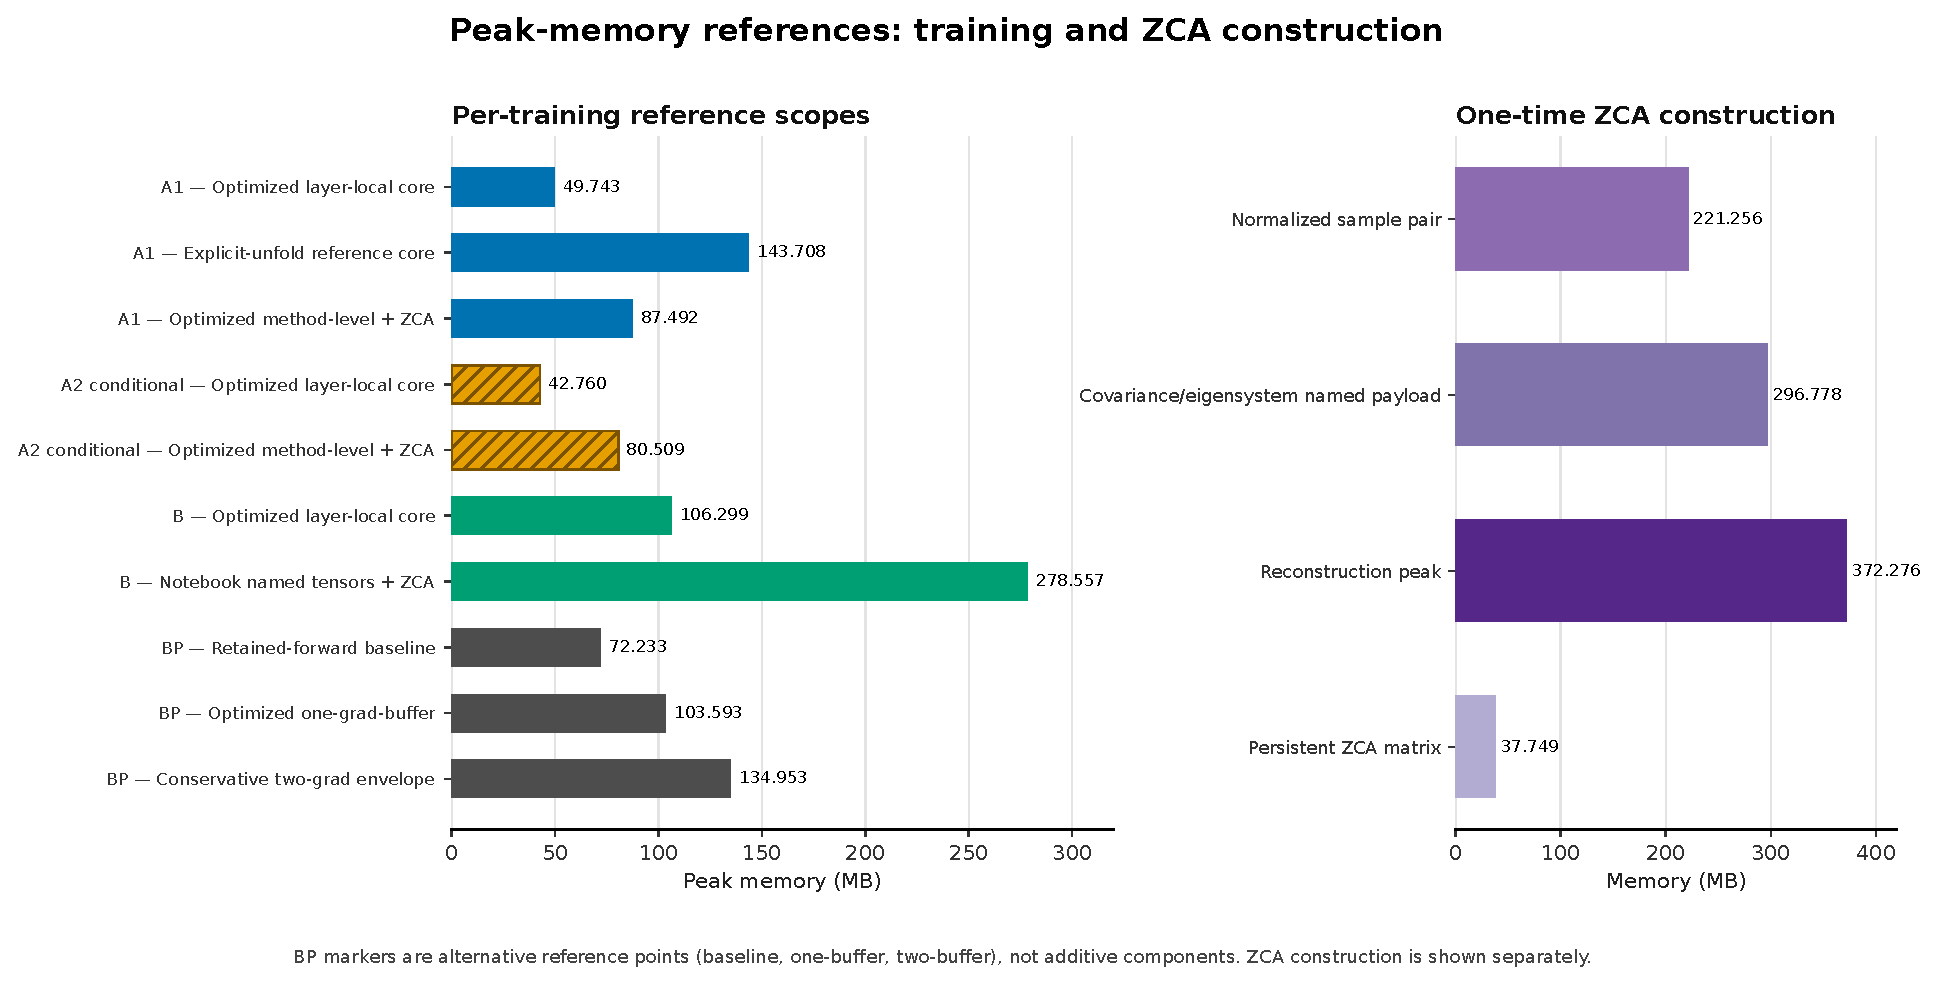
\includegraphics[width=0.92\linewidth]{fig05_memory_peak_and_zca}
    \caption{Left: analytical per-training peak tensor-payload references for A1, A2 conditional, B, and BP. Right: separate one-time ZCA construction payloads. BP points are alternative references, not additive components.}
    \label{fig:memory_peak_and_zca}
    \end{figure}
    
    The optimized layer-local core references are 49.743~MB for A1 and 42.760~MB for A2 conditional. Adding the persistent ZCA matrix gives method-level references of 87.492~MB and 80.509~MB. An explicit-unfold A1 reference reaches 143.708~MB, illustrating that direct mathematics does not guarantee a low-memory implementation if patches are materialized.
    
    B has a 106.299~MB optimized layer-local reference, while the current notebook's named tensors plus ZCA reach 278.557~MB before unknown allocator, autograd, and convolution workspaces. BP's retained-forward baseline is 72.233~MB; adding one recycled activation-gradient buffer yields 103.593~MB, and the conservative two-buffer envelope is 134.953~MB.
    
    The ZCA construction stage is larger than these ordinary training references: 221.256~MB for the normalized sample pair, 296.778~MB for the scaled-scatter/eigensystem named payload, and 372.276~MB at reconstruction. This does not mean every Hebbian batch uses 372.276~MB. Ordinary processing retains only the 37.749~MB ZCA matrix after construction.
    
    \subsection{Logical Tensor Movement}
    
    \begin{figure}[htbp]
    \centering
    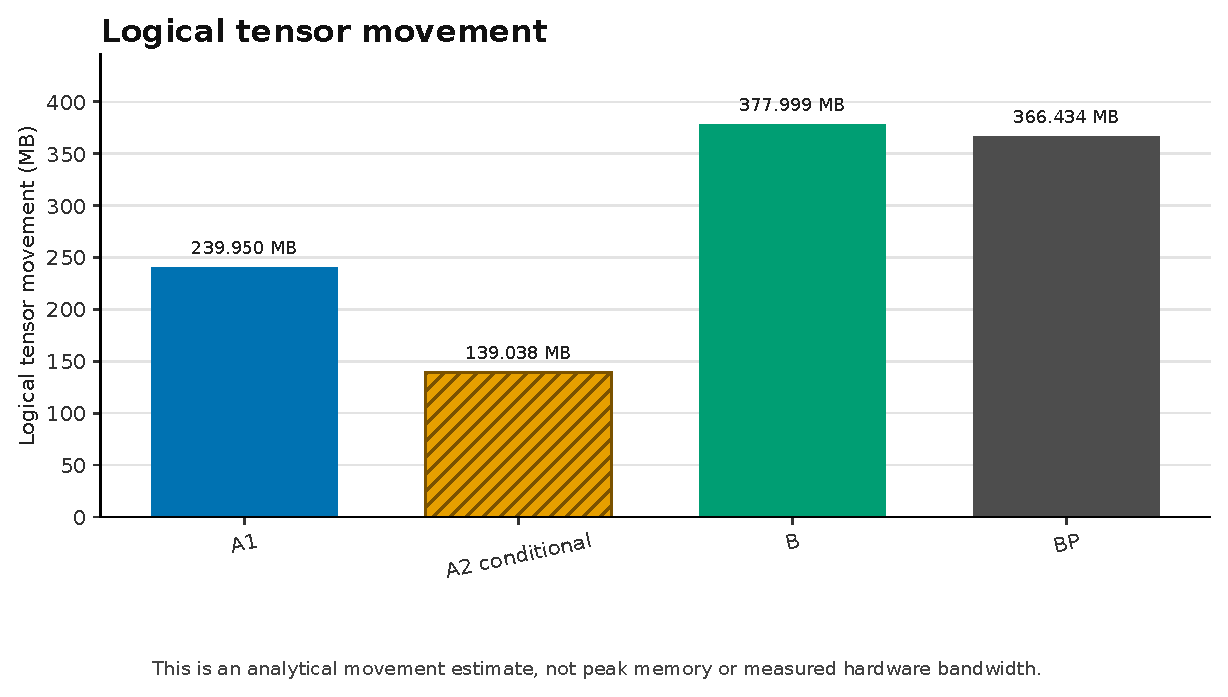
\includegraphics[width=0.85\linewidth]{fig06_logical_tensor_movement}
    \caption{Idealized logical tensor movement per compared update batch across the four studied models.}
    \label{fig:logical_tensor_movement}
    \end{figure}
    
    Table~\ref{tab:logical_movement} and Figure~\ref{fig:logical_tensor_movement} present the idealized logical tensor movement per batch.
    
    \begin{table}[htbp]
    \centering
    \small
    \caption{Idealized logical tensor movement per compared update batch.}
    \label{tab:logical_movement}
    \begin{tabular}{l r l}
    \toprule
    Method & Logical movement & Qualification \\
    \midrule
    A1 direct dense             & 239.950 MB & Representative winner-dependent reads \\
    A2 conditional sparse-aware & 139.038 MB & Requires sparse storage and kernels \\
    B surrogate/autograd        & 377.999 MB & Dense graph and gradients included \\
    BP + Adam                   & 366.434 MB & Dense backward and optimizer state included \\
    \bottomrule
    \end{tabular}
    \end{table}
    
    B's modeled logical movement is slightly above BP even though B's scalar-operation count is lower. This is a useful reminder that arithmetic and data movement are different axes. A1 and A2 conditional avoid global-gradient traffic, but their real performance would still depend on locality, fusion, cache behavior, and sparse access patterns. None of the values in Table~\ref{tab:logical_movement} is measured DRAM traffic.
    
    \section{Accuracy and Performance Context}
    
    \begin{figure}[htbp]
    \centering
    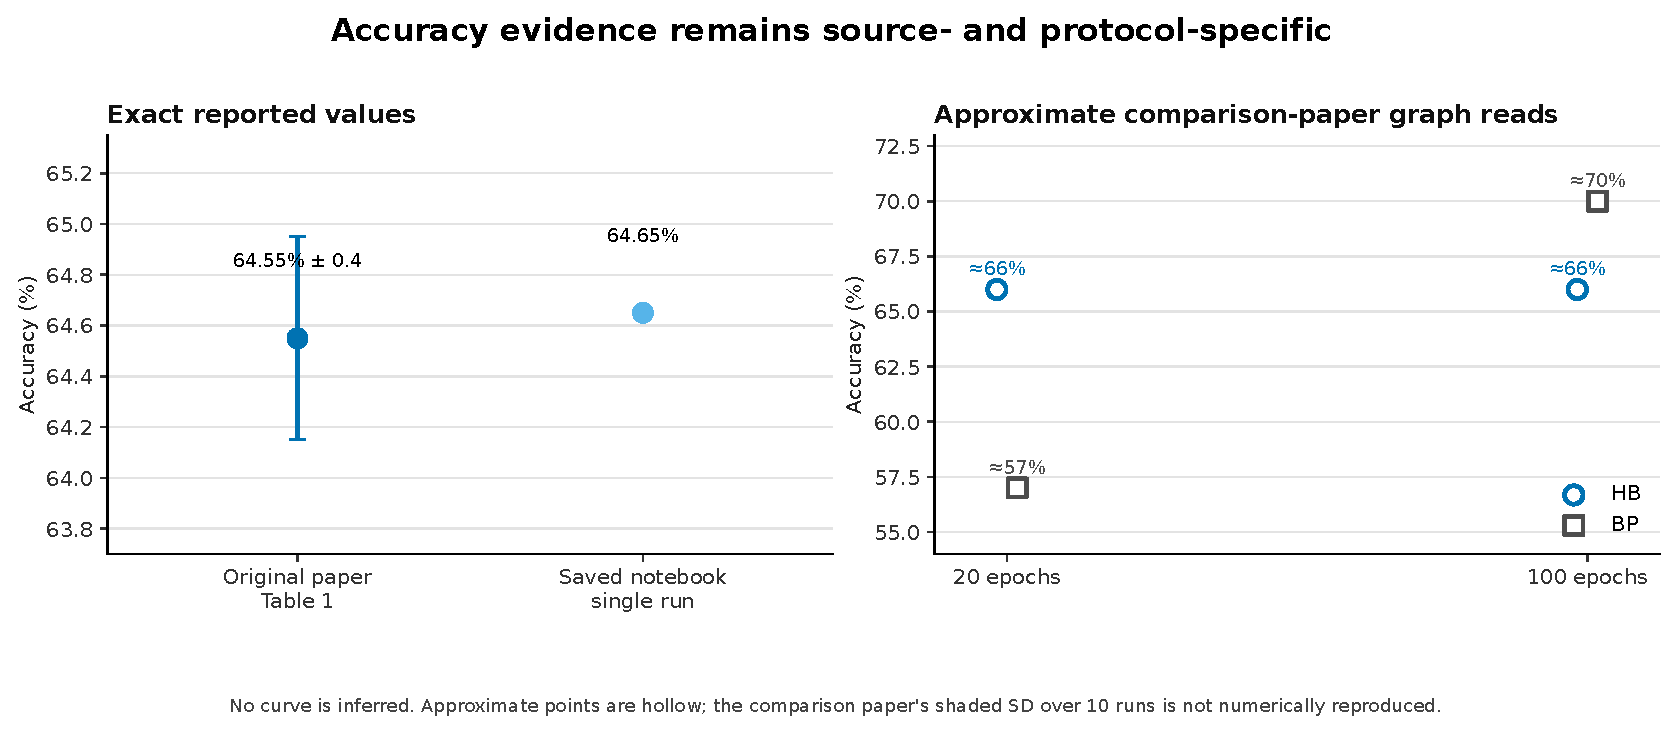
\includegraphics[width=0.88\linewidth]{fig07_accuracy_context}
    \caption{Classification accuracy across reporting sources and training regimes. Exact values from Miconi \citep{miconi2021hebbian, miconi2021repo} are shown alongside estimated empirical endpoints from the comparative evaluation by Gupta et al. \citep{gupta2023bio} (hollow markers denote visual graph estimates).}
    \label{fig:accuracy_context}
    \end{figure}
    
    To contextualize the computational cost analysis, Table~\ref{tab:accuracy_evidence} and Figure~\ref{fig:accuracy_context} summarize empirical CIFAR-10 classification accuracy across the relevant literature. Because these results stem from distinct experimental runs and reporting formats, we separate exact tabulated benchmarks from approximate graphical readings rather than conflating them into a single curve.
    
    \begin{table*}[t]
    \centering
    \footnotesize
    \setlength{\tabcolsep}{4pt}
    \renewcommand{\arraystretch}{1.2}
    \caption{CIFAR-10 accuracy evidence across reference studies.}
    \label{tab:accuracy_evidence}
    \begin{tabularx}{\textwidth}{
      >{\hsize=1.05\hsize\raggedright\arraybackslash}X
      >{\hsize=0.90\hsize\raggedright\arraybackslash}X
      c
      c
      c
      >{\hsize=1.05\hsize\raggedright\arraybackslash}X
    }
    \toprule
    Source & Method and scope & Epochs & Accuracy & Runs & Evidence class \\
    \midrule
    Miconi, Table~1 \citep{miconi2021hebbian} & Triangle + pruning, final $400\times 2\times 2$ & 20 & $64.55\% \pm 0.4$ & 10 & Exact paper table value \\
    \addlinespace
    Saved \texttt{HebbGrad\_\allowbreak Github.\allowbreak ipynb} \citep{miconi2021repo} & Default Ridge on final 1,600 features & 20 & $64.65\%$ & 1 & Exact saved run \\
    \addlinespace
    Gupta et al., Fig.~2(b) \citep{gupta2023bio} & Hebbian, 100\% data                       & 20 & $\approx 66\%$    & 10 & Approximate graph read \\
    Gupta et al., Fig.~2(b) \citep{gupta2023bio} & BP, 100\% data                            & 20 & $\approx 57\%$    & 10 & Approximate graph read \\
    \addlinespace
    Gupta et al., Fig.~2(d) \citep{gupta2023bio} & Hebbian, 100\% data                       & 100 & $\approx 66\%$   & 10 & Approximate graph read \\
    Gupta et al., Fig.~2(d) \citep{gupta2023bio} & BP, 100\% data                            & 100 & $\approx 70\%$   & 10 & Approximate graph read \\
    \bottomrule
    \end{tabularx}
    \end{table*}
    
    For the primary Hebbian CNN architecture, Miconi \citep{miconi2021hebbian} reports an average test accuracy of $64.55\% \pm 0.4\%$ across ten runs at 20 epochs (with $\pm 0.5\%$ noted in the accompanying text), aligning closely with the $64.65\%$ obtained in the reference notebook implementation \citep{miconi2021repo}. In comparative evaluations under a unified training pipeline, Gupta et al. \citep{gupta2023bio} demonstrate that 20 epochs of Hebbian training reach $\approx 66\%$ accuracy, noticeably surpassing 20-epoch backpropagation ($\approx 57\%$). Because numerical tables were not published in \citep{gupta2023bio}, these figures represent approximate readings from plotted 10-run means.
    
    Crucially, these empirical trajectories highlight a fundamental trade-off between convergence rate and asymptotic accuracy. Hebbian learning stabilizes exceptionally fast, reaching its performance ceiling within approximately five epochs ($\approx 66\%$) with negligible gains thereafter. In contrast, end-to-end backpropagation converges far more gradually, requiring up to 100 epochs to realize its full potential of $\approx 70\%$ accuracy.
    
    As a result, the substantial computational savings demonstrated in Section~8.2 (such as the $88.5\times$ reduction for A2 conditional relative to 100-epoch BP) reflect two compounding factors: the lower per-epoch cost of local Hebbian updates and the drastically shorter schedule needed to reach convergence. However, this efficiency gain involves an approximate 4 percentage point deficit in final accuracy compared to long-schedule backpropagation, showing that rapid biological stabilization prioritizes fast, resource-efficient feature acquisition over absolute terminal accuracy.
    
    \section{Discussion}
    
    \subsection{Why Direct Local Hebbian Arithmetic Can Be Lower}
    
    BP computes a forward path, gradients for the classifier and every convolutional weight tensor, input gradients needed to propagate error, activation derivatives, and Adam updates. Direct Instar does not propagate a global error. With the active top-1 cutoff and strict-positive binarization, patch contributions go to every positive channel tied at the cutoff; a location contributes to none when its maximum thresholded response is non-positive. The deterministic reference batch happened to yield exactly one such channel per spatial location. The decay term can be aggregated per filter. A layer can update before later layers learn, allowing local intermediates to be discarded.
    
    This structural difference explains why A1 is cheaper than BP even though both use dense forward convolutions. Most work in the network is still convolutional; locality does not eliminate the forward projection. It instead removes the global backward path and adaptive-optimizer arithmetic.
    
    \subsection{Optimized Direct Hebbian versus Current Autograd}
    
    The comparison between A1 and B is as important as the comparison with BP. B uses a local mathematical rule, yet it asks a general reverse-mode engine to compute the update. The one-batch B count is nearly twice A1's, and B carries dense parameter gradients. This does not make the notebook incorrect. The surrogate method is elegant, concise, and gives access to mature GPU kernels. It does show that algorithmic locality and implementation locality are not the same thing.
    
    A purpose-built implementation could exploit the direct update, layer-local liveness, and binary winner structure. Whether it would be faster on a specific GPU or CPU remains an empirical question because optimized dense libraries may outperform theoretically smaller irregular kernels.
    
    \subsection{Promise and Conditions of A2 Conditional}
    
    A2 conditional produces the lowest compute, persistent state, and logical movement in the analytical models. Layers~2 and~3 retain about one percent of their weight coordinates, so sparse execution can avoid most higher-layer multiply-accumulate work. Its 0.106~MB persistent state is particularly striking relative to dense A1, B, and BP.
    
    Those results are an opportunity estimate, not current performance. Efficient unstructured sparse convolution is difficult: indices consume space, irregular access can reduce vectorization, and conversion or load imbalance can erase theoretical savings. A credible implementation study would need sparse kernels, a specified format, end-to-end numerical validation, measured runtime and memory, and accuracy replication.
    
    \subsection{Memory Consequences of Locality}
    
    Local learning changes when information must remain live. A direct Hebbian layer can form its winner statistics and update immediately. BP must retain or reconstruct forward information for the backward pass, and Adam adds two persistent moment tensors. B retains autograd-related state despite its local rule.
    
    The results do not imply that every local algorithm has lower peak memory. The A1 explicit-unfold reference is larger than the optimized BP reference because materializing patches is expensive. Implementation strategy, not only the learning equation, determines the realized peak.
    
    \subsection{Training Budget and Accuracy Tradeoff}
    
    Cumulative compute is highly sensitive to epoch count. A five-epoch Hebbian sensitivity total can be hundreds of times below 100-epoch BP under A2 conditional. Yet the accuracy evidence shows why this ratio cannot stand alone: BP continues improving and ends above Hebbian learning in the comparison paper's full-data 100-epoch plot.
    
    For applications where early stable representations or limited training budgets matter, Hebbian learning may offer a useful operating point. For applications where the highest observed accuracy is the objective, additional BP compute may buy performance. The present evidence does not define a universal tradeoff curve because protocols, implementations, evaluation heads, and exact reported values differ.
    
    \subsection{What the Project Establishes}
    
    The strongest supported conclusion is conditional and implementation-specific. For this architecture and the frozen scalar formulas, direct local Instar requires fewer training-core operations than the equal-architecture BP reference at equal batch and equal 20-epoch scope. The current surrogate/autograd implementation also models fewer operations than BP, but the gap is smaller. Local direct execution can reduce persistent learning state, and conditional sparse execution can reduce it dramatically. These advantages persist in the broader method-level accounting.
    
    The project does not establish that Hebbian learning is the better machine-learning method. It does not measure electricity, runtime, GPU utilization, or physical memory traffic. It does not show equal accuracy at the most favorable compute ratios, and it does not implement A2 conditional. The value of the work lies in making these boundaries explicit while turning an opaque implementation comparison into a reproducible set of equations, tests, data tables, and figures.
    
    \section{Limitations}
    
    \begin{enumerate}[noitemsep]
    \item \textbf{Analytical rather than electrical measurement.} No joules, watts, runtime, or hardware-counter data were collected. Scalar operations and bytes cannot be converted directly into electricity.
    \item \textbf{Reference formulas rather than kernel instructions.} Convolution, normalization, pooling, autograd, and optimizer libraries may fuse operations or select algorithms different from the scalar expansion.
    \item \textbf{Incomplete BP specification.} Gupta et al.\ do not state BP kernels, pooling, activation, bias, loss, Adam defaults, StepLR gamma, or preprocessing. The report labels the equalization assumptions rather than attributing them to the paper.
    \item \textbf{A2 conditional.} A2 conditional assumes unstructured sparse storage and specialized kernels throughout training. It is not the behavior of the current dense notebook and has not been implemented end to end.
    \item \textbf{Representative winner statistics.} Some A1 and A2 conditional update and movement totals extrapolate the deterministic reference batch's winner pattern.
    \item \textbf{ZCA eigensolver uncertainty.} The backend and algorithm used by \texttt{torch.symeig} are not fixed. Its cost is a broad sensitivity range rather than an exact count.
    \item \textbf{Ridge implementation dependence.} Default \texttt{Ridge()} is not version-pinned. Solver choice, dtype, centering, validation, and copies can change the actual cost and memory.
    \item \textbf{Tensor payload is not allocator memory.} Peak references exclude Python objects, caching allocators, autograd bookkeeping, and many cuDNN or BLAS workspaces.
    \item \textbf{Logical movement is not physical DRAM traffic.} The movement model assumes idealized passes and reuse. Cache lines, tiling, fusion, and sparse access determine actual traffic.
    \item \textbf{Approximate comparison-paper accuracy.} Four CIFAR-10 endpoints are visual reads from plotted means. Their numerical standard deviations cannot be recovered from shading.
    \item \textbf{Protocol differences.} The active notebook, original paper, comparison paper, and BP reference differ in preprocessing, learning rates, readout, and other details. Compute totals and accuracy values are therefore contextual rather than one controlled benchmark.
    \item \textbf{Stochastic saved notebook.} The saved 64.65\% result is one run. The test transform includes random horizontal flipping, and adaptive thresholds continue changing during feature collection.
    \item \textbf{ZCA construction difference.} The original paper states that ZCA uses the full training set; the active notebook uses one shuffled 9,000-image batch. It also computes $\mathbf{T}^T \mathbf{T} / 3072$, dividing by the feature count rather than the 9,000 samples, so the construction is a scaled scatter matrix rather than a conventional sample covariance. The method-level model follows the active code, and this terminology correction changes no frozen total.
    \item \textbf{Limited equivalence claim.} The deterministic test verifies one representative post-burn-in batch and active branches. It does not reproduce complete training or accuracy for A1 or A2 conditional.
    \end{enumerate}
    
    \section{Conclusion}
    
    This project investigated the computational and memory implications of a concrete Hebbian convolutional network rather than making a general biological or performance claim. The notebook's surrogate loss was shown algebraically to encode Grossberg Instar, and a deterministic test found numerically identical direct and autograd updates for all three layers on the tested batch. This justified separating the mathematics of local learning from the cost of its current framework implementation.
    
    Under the frozen analytical model, A1 direct dense, A2 conditional sparse-aware, and B surrogate/autograd all require fewer training-core scalar operations than the equal-architecture BP reference at matched batch and 20-epoch scopes. Direct execution also reduces persistent state by eliminating parameter gradients and Adam moments; A2 conditional offers the largest resource savings if sparse storage and kernels are genuinely available. The full method-level analysis, including known ZCA and Ridge work, preserves the same ordering.
    
    These results answer the research question with an important qualification: direct local Hebbian learning has a clear modeled resource advantage for this architecture, but that advantage is not evidence of measured energy reduction or overall learning superiority. The accuracy sources are not protocol-identical, and the most favorable five-versus-100-epoch comparison is a convergence sensitivity rather than an equal-accuracy result. A future hardware experiment should implement A1 and A2 conditional, hold the training and evaluation protocol fixed, measure runtime, allocator peak, DRAM traffic, and energy, and report accuracy distributions over repeated runs. Until then, the present report provides a rigorous hardware-independent baseline and an explicit map of what remains to be tested.
    
    \section*{Reproducibility and Artifact Map}
    
    The report is grounded in the following frozen project artifacts:
    \begin{itemize}[noitemsep]
    \item Architecture and code audit: \texttt{mathematical\_\allowbreak architectural\_\allowbreak audit.md};
    \item Deterministic update check: \texttt{direct\_\allowbreak hebb\_\allowbreak equivalence\_\allowbreak test.py};
    \item Hebbian arithmetic: \texttt{hebbian\_\allowbreak compute\_\allowbreak cost.py};
    \item BP definition and smoke test: \texttt{backprop\_\allowbreak reference.py};
    \item BP arithmetic and matched comparisons: \texttt{backprop\_\allowbreak compute\_\allowbreak cost.py};
    \item Full-pipeline arithmetic: \texttt{method\_\allowbreak level\_\allowbreak compute\_\allowbreak cost.py};
    \item Memory and movement: \texttt{memory\_\allowbreak resource\_\allowbreak cost.py};
    \item Accuracy evidence classification: \texttt{accuracy\_\allowbreak performance\_\allowbreak context.md};
    \item Graph source data: \texttt{results/data/*.csv}; and
    \item Frozen figures: \texttt{results/figures/*}.
    \end{itemize}
    All figures used in this report are generated from the CSV source tables. The original notebooks remain unmodified.
    
    \bibliographystyle{unsrtnat}
    \bibliography{references}
    
    \end{document}